\documentclass[conference]{IEEEtran}
\usepackage{graphicx}
\usepackage[a4paper, margin=1cm]{geometry}
%\usepackage{times} % Uncomment to use the Times font
\usepackage{tikz}
\usepackage{titlesec} 
\usepackage{array}
\usepackage{colortbl} 
\usepackage{fancyhdr}
\usepackage{authblk}
\usepackage{amsmath}
\usepackage{hyperref}
\usepackage[english]{babel}
\usepackage[square, numbers]{natbib} 
\usepackage[nottoc]{tocbibind}

\bibliographystyle{abbrvnat}

\definecolor{headercolor}{rgb}{0.8, 0.8, 0.8}
\definecolor{rowcolor}{rgb}{1, 1, 0.6}
\definecolor{overallcolor}{rgb}{1, 0.8, 0.3}

\setlength{\columnsep}{0.5cm} 

\title{Bioactivity Prediction by a Heterogeneous Siamese Neural Network (SNN)}

\author{Pham Hai Nam, Nguyen Son, Doan Huu Thanh, Le Mau Minh Phuc*}
\affil{* University of Science and Technology of Hanoi}

\begin{document}
\maketitle
\begin{abstract}
  The Bioactivity Determination while taking medicine causes challenges leading to drug failure. To address this risk and enhance compound activities, Bioactivity Classes during lead optimization are necessary based on the foundation of Structure-activity Relationships as the connection between the Chemical Compounds and the Bioactivity. This study has two major objectives: (i) to evaluate the BioAct-Het (A Siamese Neural Network) model by taking 7 predicted and actual side-effects drugs according to evaluation metrics to ensure the trustworthiness and (ii) to find the Bioactivity Classes of 24 marketed drugs, including both COVID-19 and non-COVID-19 substances, through BioAct-Het. Since the confirmation of trustworthiness of BioAct-Het results in greater than 75\%, the model is believed to be an accurate model. It is moreover used to examine and analyze the results of 25 drug inputs. Therefore, 5 drugs are both concluded as at least side effects and requiring careful use, leading to some particular side effects including immune system disorders, vascular disorders, nervous system disorders, metabolism and nutrition disorders, and others. Last but not least, with these concluded drugs, Paxlovid (Nirmatrelvir) and Interferon-beta 1a (IFN-$\beta$1a) are recommended for use in COVID-19 treatment combined with the prescription of doctors. The data and code for this study are available on \url{https://github.com/Xernnn/Bioact-Pred-Het-SNN}. However, the datasets were obtained from publicly available sources.
\end{abstract}

\textbf{Keywords:} BioAct-Het, Bio-Prof, bioactivity, drug side-effects, Siamese neural networks, COVID-19 treatment, structure-activity relationships.

% Introduction
\section{Introduction}
\subsection{Context of Computational Methods in Drug Discovery}
The drug-likeness of a compound must be identified and optimized with a demanding and lengthy process \cite{Wouters}. Generally, it takes over a decade and costs billions to bring a new chemical compound to market as a drug. Predicting a compound's bioactivities, which relies on the effects of living organisms including both positive and negative outcomes like side effects and toxicity, is crucial in drug discovery. During lead optimization, the objective is to improve the structure of leads while maintaining the therapeutic properties to enhance bioactivity \citet{Hughes}.\\

However, experimental evaluation related to bioactivity is challenging due to the number of potential analogs and the high screening costs \citet{Reymond}. Computational techniques, to explore the structure-activity relationship (SAR) with demonstrated compounds with similar structures often share bioactivities, are a viable alternative to expensive screening methods at laboratories \citet{Nantasenamat}.\\

Application of computation methods to predict the bioactivity of novel compounds encounters two challenges, including compound representation and data scarcity. Compound representation, firstly, involves selecting an appropriate structure representation. SMILES, fingerprints, and graphs with traditional algorithms have been used to represent a compound in the bioactivity class \citet{Weininger}. Moreover, the lack of data scarcity to train a reliable model necessitates the creation of varied datasets consisting of chemical substances with a range of bioactivities. Ratios that are out of balance between positive and negative data can also impact the performance of prediction. Torres et al. introduced an additional one-shot classification approach using a Siamese neural network architecture, which employs a Convolutional Neural Network (CNN) to identify novel compound features, particularly for less-represented classes. This model, with the use of the Tox21 database, represents compounds using the one-hot encoding of canonical SMILES structures and make into groups based on chemical structures for training \citet{Weininger}.\\

The bioactivity class prediction (BCP) problem can be addressed by many research methods that rely on the central hypothesis of SAR studies. These approaches aim to identify patterns in drug chemical structures associated with specific bioactivity classes and can be trained on pairs of compounds sharing the same bioactivity class to learn similarities and pairs with bioactivities to obtain the differences, and used to predict whether new chemical compounds belong to which particular bioactivity class \citet{Vella}\\

The evaluation of previous studies demonstrates that the relationship between chemical compounds and bioactivities is extremely complex due to a significant relationship challenge in the BCP problem. To address these difficulties, this study implements a method called BioAct-Het, which attempts to determine the likelihood of association between a compound and a bioactivity class. BioAct-Het uses a heterogeneous SNN to map chemical compounds and bioactivity classes into a unified latent space, which is capable of representing bioactivity classes based on related substances. The performance of BioAct-Het is evaluated using both supervised learning and meta-learning approaches on three databases: SIDER, Tox21, MUV, and the self-constructed dataset \citet{Heyrati}.\\
\subsection{Related Work}
BioAct-Het is a heterogeneous SNN (Siamese Neural Network) that solves the bioactivity class prediction problem, meaning whether the compound causes the bioactivity or not. The input of the model consists of two branches, which are embedding compounds and bioactivity classes. Since this is a binary classification, the output will be 1 if the compound causes the bioactivity class, otherwise, the prediction will be 0.\\

\subsubsection{Chemical representation as feature extractors - Graph Convolutional Networks (GCN)}
In the experiment protocol, Graph Convolutional Networks (GCN) are used to represent the chemical structure of the compounds, which is one of the two inputs for the BioAct-Het architecture. Initially, the SMILES structure of these compounds is transformed into graph representations, where each node corresponds to an atom, and the edges represent the bonds between these atoms \citet{Li}. The graphs are then passed into the GCN to represent the chemical structures of the compounds as vectors.\\

The GCN architecture contains two operations, the first one involves calculating the weighted sum of the representations of nodes in a graph. The sum is then processed through a linear layer following a sigmoid function. The second operation is to use an element-wise maximum to the representations of nodes in a graph, which is then passed through a Multilayer perceptron for the final vector representations of a chemical compound. For this process, two pre-trained models are carried out: GCN-Canonical GCN-AttentiveFP \citet{Heyrati}.\\

GCN-Canonical gets the information from the nodes and the following neighbors by considering how many connections or degrees each node has. The method ensures that every node is calculated equally based on the number of connections to the other nodes \citet{Kipf}. On the other hand, GCN-AttentiveFP is used to identify the important connections between any nodes, while still keeping the layout of the molecule. The model is designed to capture critical relationships in the molecular structures \citet{Xiong}.\\

\subsubsection{Bio-Prof as a bioactivity class model}
The Bio-Prof model is used to represent the bioactivity classes based on the substructures of the chemical compounds, which is the other input of BioAct-Het. To represent the bioactivity classes, the Morgan fingerprint, a binary string representation encoding function, is used for this purpose by examining which molecule structures in the compounds that are known to be active or inactive to the bioactivity classes. Each bit in the fingerprint represents the presence or absence of a particular substructure within a compound for each bioactivity class \citet{Morgan}.\\

\subsubsection{BioAct-Het as a bioactivity prediction model}
As previously mentioned, BioAct-Het is a heterogeneous SNN (Siamese Neural Network), which is different from homogeneous SNNs, in which the inputs are dual-branch networks with tied weights. Heterogeneous SNN consists of distinctive networks in two various branches and a different learning component. The branches transform the initial representation of the chemical compounds and bioactivity classes into a unified latent space to share properties and become comparable. To bring the similarity of bioactivity classes and chemical compounds close together in the latent space, BioAct-Het calculates the likelihood of association through the distances \citet{Bemis}.\\

First of all, by taking the results from the GCN models and the Bio-Prof model, BioAct-Het passes the results to the dense layers containing two nonlinear functions, ReLU as the activation functions and kl-divergence loss functions. The aim is to transform chemical compound embedding vectors and bioactivity class embedding vectors into having the same dimension, creating a unified latent space for chemical compounds and bioactivities to produce a distribution.\\

In the second step, BioAct-Het predicts the association between the compound and bioactivity class based on the distance in the latent space. The distance vector is then passed through a dense layer containing a nonlinear function, ReLU as the activation function and sigmoid function with a threshold of 0.5. Since the output layer contains one node, the result will be 1 if the compound causes the bioactivity class, otherwise, the prediction will be 0, with the loss function being binary cross-entropy function. After that, minimizing the loss function is required to increase the model’s effectiveness in predictions \citet{Wu}.\\

\subsection{Our Contribution}
The study of marketed drugs and COVID-19 side-effect drugs is relatively time-consuming and difficult due to a large range of biological knowledge. Moreover, even though it is available on GitHub under \url{https://github.com/Xernnn/Bioact-Pred-Het-SNN}, the source code needs to be improved and re-implemented to evaluate available side-effect drugs in SIDER and predicted side-effect drugs according to confusion metrics. This study is mostly to understand the application of machine learning in Medicine and case studies of COVID-19, instead of only conventional paths, such as training and testing a type of datasets on the internet, and conclude. We, therefore, spent time studying medical cases and new neural network cases that have an objective to real-life applications with a clear further study collaborated with virtual screening. \\

In detail, the main contributions of this study:
\begin{itemize}
  \item To construct an experimental design with the relation of SAR.
  \item To construct the dataset with the study of which marked drugs treating COVID-19.
  \item To evaluate the model, which considers a compound-bioactivity class pair as a positive pair and a negative pair, with the complex relationship between compounds and bioactivity classes, to learn a unified latent space via a heterogeneous SNN.
  \item To visualize the outcome to further study.
\end{itemize}


\section{Methods - Experimental Design}
The design of each experiment is to predict whether marketed drugs cause some bioactivity classes. This computational model is used initially to forecast the potential bioactivities of marketed drugs before starting with virtual screening or docking studies.\\

In Figure 1, potential drugs are chosen with the self-constructed dataset treating COVID-19. Moreover, it goes to pre-trained chemical compounds - GCN-AttentiveFP model (feature extractors) to get chemical representations. These representations are then fed to the BioAct-Het model, linked to each side effect class representation that was gained. The model results in the probability of each drug showing side effect classes in the form of embedding vectors in the range of 0 to 1. If the probability is greater than 0.5, the bioactivity class is represented in chemical compounds and vice versa \citet{Shih}.

\begin{figure}[htbp]
  \centering
  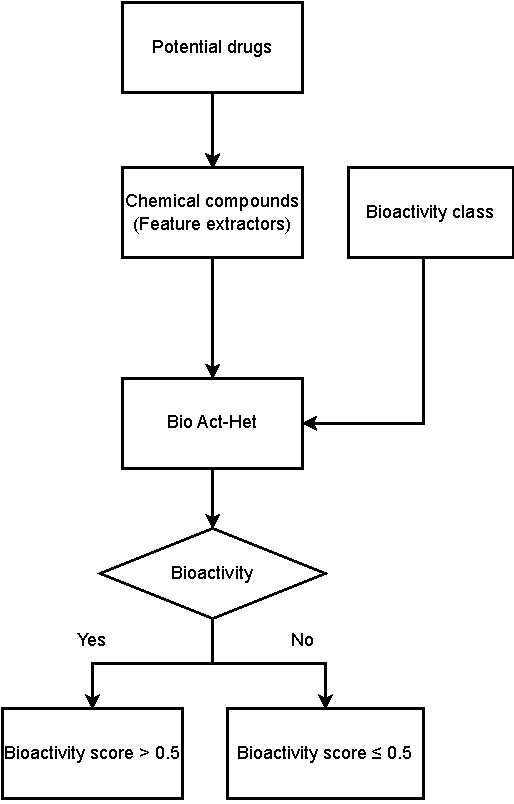
\includegraphics[width=0.3\textwidth]{flowchart.pdf}
  \caption{Flowchart}
\end{figure}

\subsection{Data materials}
There are four different datasets for distinct purposes related to side effects, toxicity, and the risk of overfitting to similar compounds. Almost all datasets are used as pre-trained models for less time-consuming re-training processes, while a manual collection dataset is used for testing the model to further analyze results. Table 1 describes the ratios for training and testing equivalent to each dataset.\\

\subsubsection{A manual collection dataset}
A manual collection dataset is constructed to evaluate the pre-trained model and analyze the further results. It contains 24 marketed drugs with the SMILES structure used to treat COVID-19. These drugs are used to evaluate the model by selecting 7 selected drugs with the 27 side effects in SIDER compared with the prediction of these 7 drugs of an SNN model. Moreover, potential side effects extracted from results can be used to propose which side effects are typical for dosage use and chemical compound recommendations. Details in Appendix 1.\\

\subsubsection{SIDER}
The SIDER is a dataset of marketed-drugs side effects. These include 27 classes using Medical Dictionary for Regulatory Activities (MedDRA) classification according to system organ classes. SIDER is a variant in, for example, Hepatobiliary disorders, Metabolism and nutrition disorders, and Product issues. Details in Table 1.\\

\subsubsection{Tox21}
Tox21 is designed to evaluate the toxicity of chemical substances. It consists of 12 toxicological assays following receptors, which forecast the potential risks linked to exposure to these compounds. Details in Table 1.\\

\subsubsection{MUV}
The MUV is indicated as a benchmark for evaluating the performance of virtual screening with 17 challenging tasks and priority of the minimization of the risk of overfitting to similar compounds. Details in Table 1.

\begin{table}[h!]
  \centering
  \caption{SIDER, Tox21, MUV datasets information}
  \label{tab: SIDER, Tox21, MUV Datasets}
  \begin{tabular}{|c|c|m{1.3cm}|c|c|}
    \hline
    \rowcolor{headercolor}
    \textbf{Dataset} & \textbf{Compounds} & \multicolumn{1}{|c|}{\textbf{Bioactivity Classes}} & \textbf{(+) Samples} & \textbf{(-) Samples} \\ \hline
    \textbf{SIDER}   & 1427               & 27                                                 & 21,868               & 16,661               \\ \hline
    \textbf{Tox21}   & 7831               & 12                                                 & 5,862                & 72,084               \\ \hline
    \textbf{MUV}     & 93,087             & 17                                                 & 489                  & 1,332,593            \\ \hline
  \end{tabular}
\end{table}

\subsection{Data representation and pre-trained BioAct-Het Model}
As described in related work, GCN-Canonical and GCN-AttentitiveFP are used for feature extractors. Chemical compound representation steps are then gone into Bio-Prof which is based on the profile of chemical structure of related compounds. Moreover, the model called BioAct-Het (a heterogeneous SNN) plays a role in bringing the similar concept of bioactivity classes and chemical compounds in the latent space and inferring the likelihood of association through distances as embedding vectors. \\

The strategies and evaluation approach in pre-trained models are according to Table 2.\\

\begin{itemize}
  \item The association-based strategy is to determine the relationship between a chemical substance in the data set and a bioactivity class (preferred to use in BioAct-Het).
  \item The bioactivity class-based strategy aims to uncover chemical compounds that demonstrate new and uncommon bioactivity (preferred to use in Bioactivity class).
  \item The compound-based strategy is to predict the bioactivity classes of a newly found chemical compound released into the market (preferred to use in Chemical Compounds - feature extractors).
\end{itemize}

\begin{table}[h!]
  \caption{Caption here}
  \label{tab:your_label_here}
  \centering
  \begin{tabular}{|m{2.2cm}|c|c|m{2.8cm}|}
    \hline
    \rowcolor{headercolor}
    \multicolumn{1}{|c|}{\textbf{Category}}        & \multicolumn{1}{c|}{\textbf{Training}} & \multicolumn{1}{c|}{\textbf{Testing}} & \multicolumn{1}{c|}{\textbf{Purpose}}                                \\ \hline
    Association-based \newline (Pre-trained)       & 90\%                                   & 10\%                                  & Predict the unknown \newline association                             \\ \hline
    Bioactivity-based \newline (Pre-trained)       & 80\%                                   & 20\%                                  & Identify chemical compounds that exhibit a novel type of bioactivity \\ \hline
    Compound-Based Strategy \newline (Pre-trained) & 90\%                                   & 10\%                                  & Predict the bioactivity classes of a newly found chemical compound   \\ \hline
  \end{tabular}
\end{table}

\subsection{Evaluation Metrics}
Confusion matrices and other evaluation metrics are used to assess how accurate the model is. These tools are essential for determining the trustworthiness of the model and for further analysis.

\[
  \text{Accuracy} = \frac{\text{TP} + \text{TN}}{\text{TP} + \text{TN} + \text{FP} + \text{FN}}
\]

\[
  \text{Precision} = \frac{\text{TP}}{\text{TP} + \text{FP}}
\]

\[
  \text{Recall} = \frac{\text{TP}}{\text{TP} + \text{FN}}
\]

\[
  \text{F1 Score} = 2 \cdot \frac{\text{Precision} \times \text{Recall}}{\text{Precision} + \text{Recall}}
\]

\begin{table}[h!]
  \centering
  \caption{Example of a 5x2 Table}
  \label{tab:Prediction_Definition}
  \begin{tabular}{|>{\raggedright\arraybackslash}p{2.5cm}|>{\raggedright\arraybackslash}p{6cm}|}
    \hline
    \rowcolor{headercolor}
    \multicolumn{1}{|c|}{\textbf{Prediction}} & \multicolumn{1}{c|}{\textbf{Definition}}                                                         \\ \hline
    \textbf{True Positive (TP)}               & The number of activated bioactivity classes for a drug predicted correctly by the BioAct-Het.    \\ \hline
    \textbf{True Negative (TN)}               & The number of nonactivated bioactivity classes for a drug predicted correctly by the BioAct-Het. \\ \hline
    \textbf{False Positive (FP)}              & The number of activated bioactivity classes for a drug predicted wrongly by the BioAct-Het.      \\ \hline
    \textbf{False Negative (FN)}              & The number of nonactivated bioactivity classes for a drug predicted wrongly by the BioAct-Het.   \\ \hline
  \end{tabular}
\end{table}


\section{Results and Evaluation}
\subsection{Model Evaluation}
To evaluate the performance of the BioAct-Het model, a testing process is carried out. This involves comparing the side effects of 7 actual drugs from the SIDER dataset with those predicted for 7 drugs, among a total of 25 potentially marketed drugs that had ground truth side-effect labels. These results are presented in Table N.
These drugs were:\\[6pt]


For each drug-side effect pair in the test set, the model made a prediction between 0 and 1 for the likelihood of that side effect occurring. The threshold for classifying predictions is 0.5, which is a positive prediction for the side effects if the result is above the threshold, and below the threshold results in a negative prediction.\\

We then generated bubble charts and confusion matrices to visualize how well the model's predictions matched each drug's ground truth labels. The bubble charts showed the counts of true positive, false positive, true negative, and false negative predictions for each drug. Overall, the confusion matrices indicated the model accurately predicted both the presence and absence of side effects for most drug-side effect pairs. (Appendix 2)\\

To quantify the model's performance, the evaluation metrics are being used, such as accuracy, precision, recall, and F1 score calculation based on the true and false positives and negatives. The accuracy was 85.7\%, precision was 86.2\%, recall was 85.3\%, and F1 score was 85.7\%. All of these evaluation metrics were well above the 75\% threshold, demonstrating the model could reliably predict side effects in a one-shot learning scenario.

\begin{table}[h!]
  \centering
  \caption{Model Evaluation with 7 Testing Drugs}
  \label{table:evaluation}
  \begin{tabular}{|c|c|c|c|c|}
    \hline
    \rowcolor{headercolor}
    \textbf{Drug Name}          & \textbf{Accuracy} & \textbf{Precision} & \textbf{   Recall   } & \textbf{F1 Score} \\ \hline
    \rowcolor{rowcolor}
    \textbf{Chloroquine}        & 85.71\%           & 88.57\%            & 85.71\%               & 85.08\%           \\ \hline
    Famotidine                  & 89.29\%           & 92.50\%            & 89.29\%               & 89.82\%           \\ \hline
    Guanfacine                  & 96.43\%           & 93.05\%            & 96.43\%               & 94.69\%           \\ \hline
    \rowcolor{rowcolor}
    \textbf{Hydroxychloroquine} & 78.57\%           & 76.07\%            & 78.57\%               & 77.26\%           \\ \hline
    \rowcolor{rowcolor}
    \textbf{Oseltamivir}        & 85.71\%           & 82.77\%            & 85.71\%               & 83.99\%           \\ \hline
    Prednisolone                & 82.14\%           & 79.01\%            & 82.14\%               & 79.79\%           \\ \hline
    \rowcolor{rowcolor}
    \textbf{Ritonavir}          & 96.43\%           & 92.99\%            & 96.43\%               & 94.68\%           \\ \hline
    \rowcolor{overallcolor}
    \textbf{Overall}            & \textbf{87.76\%}  & \textbf{85.42\%}   & \textbf{87.76\%}      & \textbf{86.52\%}  \\ \hline
  \end{tabular}
\end{table}

Ritonavir’s confusion matrix, for example, is represented in figure 2 and 3, it is clear to notice the distribution of true positive and false negative is relatively significant enough to make this model accurate.\\

\begin{figure}[htbp]
  \centering
  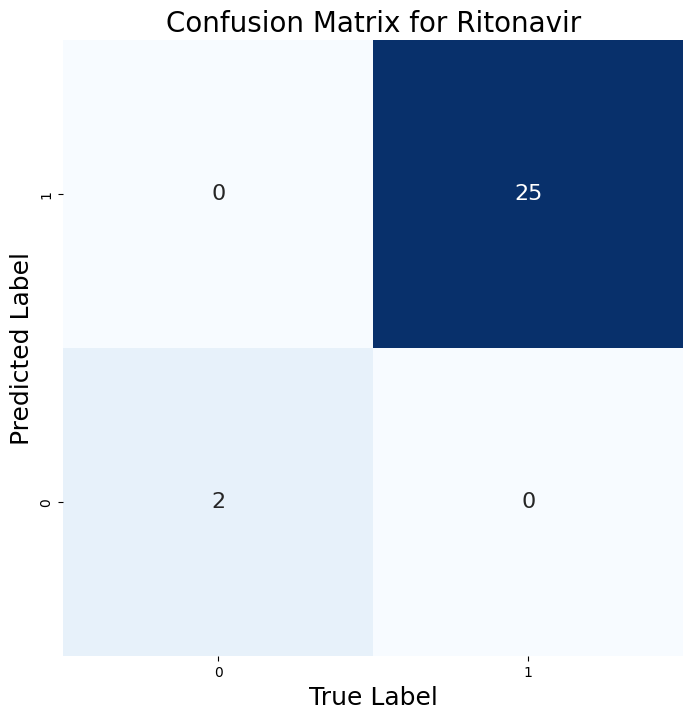
\includegraphics[width=0.35\textwidth]{C:/Users/stdso/Documents/USTH/Med/BioAct-Het-main/Output/CF/Ritonavir_confusion_matrix.png}
  \caption{Ritonavir Confusion Matrix}
  \label{fig:Ritonavir Confusion Matrix}
\end{figure}

\begin{figure}[htbp]
  \centering
  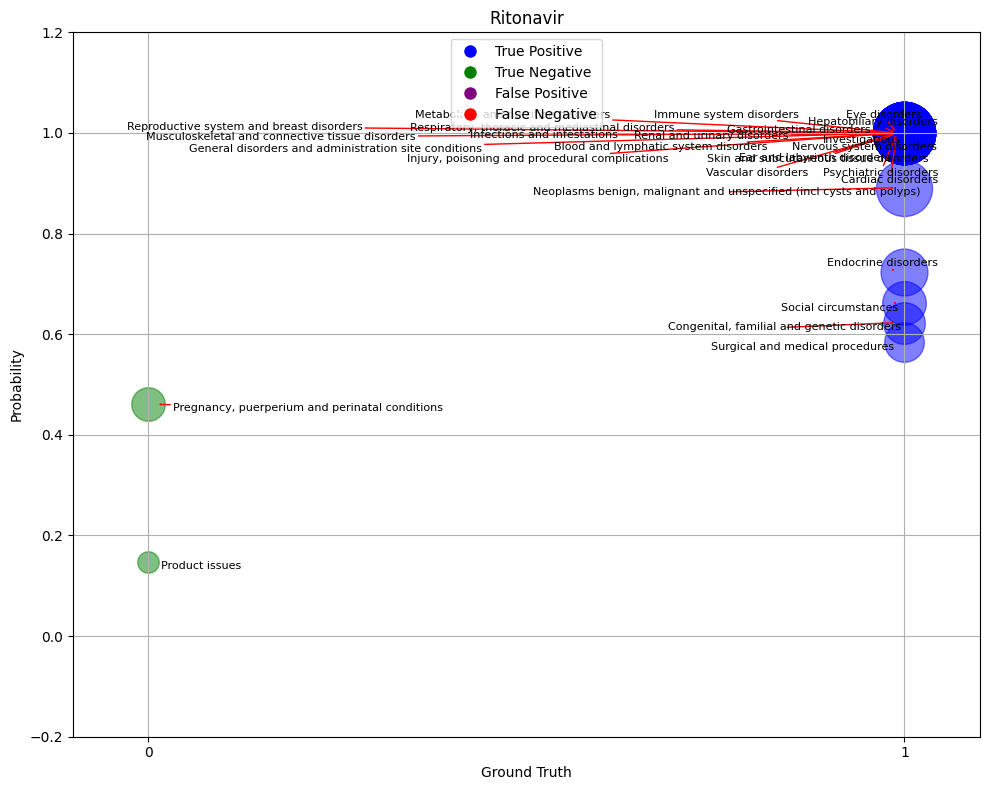
\includegraphics[width=0.5\textwidth]{C:/Users/stdso/Documents/USTH/Med/BioAct-Het-main/Output/Bubble/Ritonavir_bubble_chart.png}
  \caption{Ritonavir Confusion Matrix}
  \label{fig:Ritonavir Bubble Chart}
\end{figure}

Notably, through table N, four of the drugs tested - Hydroxychloroquine, Oseltamivir , Chloroquine and Ritonavir - are currently used as COVID-19 treatments, and the model achieved especially high scores on these drugs. \textit{This suggests the model may be particularly suited for evaluating potential COVID-19 drug candidates.}\\

\subsection{Drug Discovery Results Analysis}
Next, to investigate the safest drug options, an identification process is carried out, which results in the 5 predicted drugs having the fewest side effects by the model:

\begin{itemize}
  \item \textbf{Paxlovid (Nirmatrelvir)} with \textbf{12} predicted side effects.
  \item \textbf{Linagliptin} with \textbf{11} predicted side effects.
  \item \textbf{Interferon-beta-1a} with \textbf{11} predicted side effects.
  \item \textbf{Famotidine} with \textbf{10} predicted side effects.
  \item \textbf{Hydroxychloroquine} with \textbf{10} predicted side effects.
\end{itemize}

\noindent
\begin{center}
  \begin{tabular}{p{0.20\textwidth} p{0.20\textwidth}}
    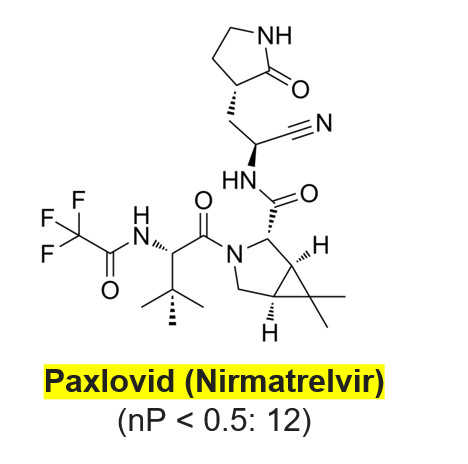
\includegraphics[width=\linewidth]{C:/Users/stdso/Documents/USTH/Med/BioAct-Het-main/Output/Least/Paxlovid.jpg}           & 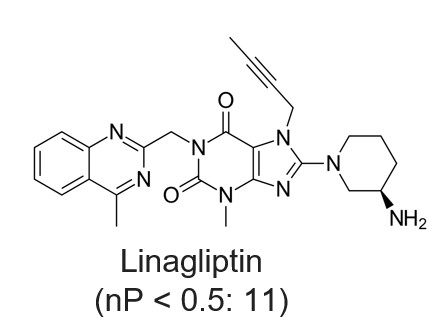
\includegraphics[width=\linewidth]{C:/Users/stdso/Documents/USTH/Med/BioAct-Het-main/Output/Least/Linagliptin.jpg} \\
    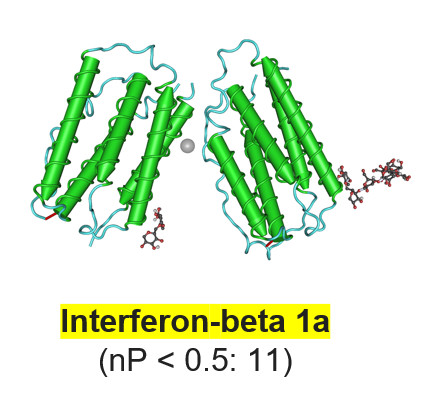
\includegraphics[width=\linewidth]{C:/Users/stdso/Documents/USTH/Med/BioAct-Het-main/Output/Least/Interferon-beta-1a.jpg} & 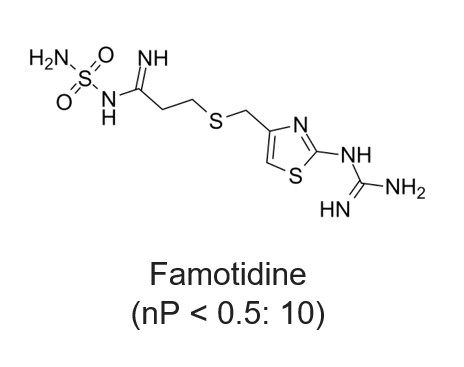
\includegraphics[width=\linewidth]{C:/Users/stdso/Documents/USTH/Med/BioAct-Het-main/Output/Least/Famotidine.jpg}  \\
  \end{tabular}

  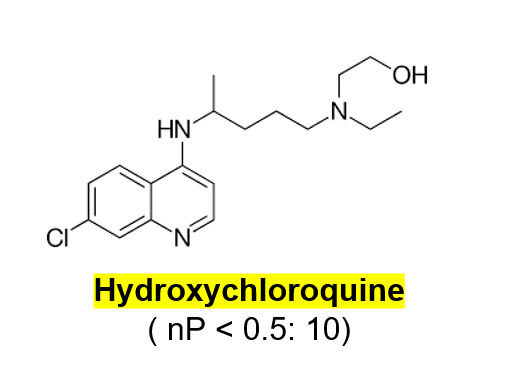
\includegraphics[width=0.4\linewidth]{C:/Users/stdso/Documents/USTH/Med/BioAct-Het-main/Output/Least/Hydroxychloroquine.jpg} \\
\end{center}

Paxlovid, Interferon-beta-1a, and Hydroxychloroquine are relevant to treating COVID-19. Therefore, these three drugs will be the focus of the next stage of analysis. However, Hydroxychloroquine is reported as an untrusted drug due to a wide range number of side effects. Therefore, only Paxlovid and Interferon-beta-1a are issued to select as the potential drugs to treat COVID-19 disease.\\

On the other hand, the 5 drugs predicted to have the most side effects, over 20 each, were:

\begin{itemize}
  \item \textbf{Umifenovir} with \textbf{21} predicted side effects.
  \item \textbf{Prednisolone} with \textbf{22} predicted side effects.
  \item \textbf{Ritonavir} with \textbf{25} predicted side effects.
  \item \textbf{Cyclosporine} with \textbf{26} predicted side effects.
  \item \textbf{Ivermectin-B1a} with \textbf{26} predicted side effects.
\end{itemize}

\noindent
\begin{center}
  \begin{tabular}{p{0.20\textwidth} p{0.20\textwidth}}
    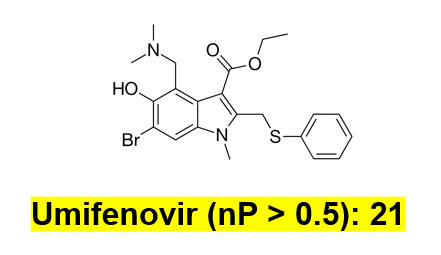
\includegraphics[width=\linewidth]{C:/Users/stdso/Documents/USTH/Med/BioAct-Het-main/Output/Most/Umifenovir.jpg} & 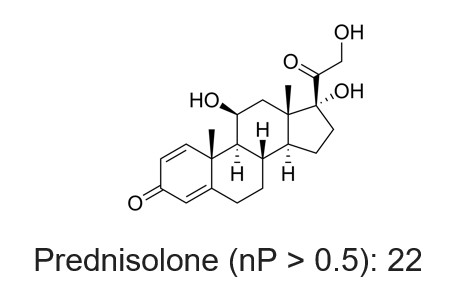
\includegraphics[width=\linewidth]{C:/Users/stdso/Documents/USTH/Med/BioAct-Het-main/Output/Most/Prednisolone.jpg} \\
    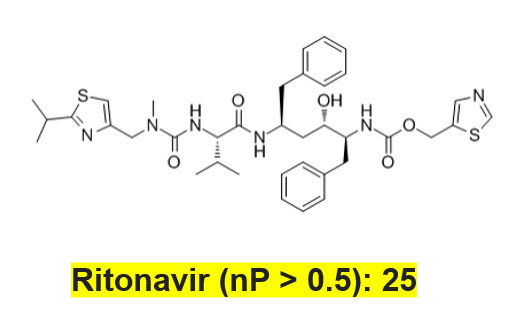
\includegraphics[width=\linewidth]{C:/Users/stdso/Documents/USTH/Med/BioAct-Het-main/Output/Most/Ritonavir.jpg}  & 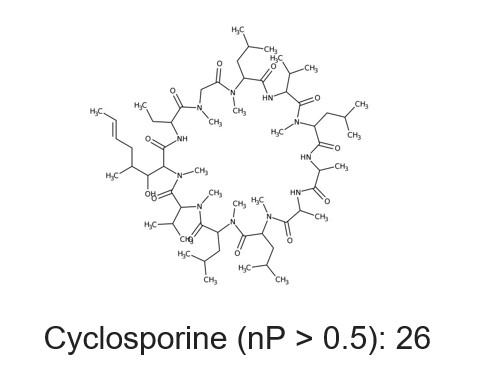
\includegraphics[width=\linewidth]{C:/Users/stdso/Documents/USTH/Med/BioAct-Het-main/Output/Most/Cyclosporine.jpg} \\
  \end{tabular}

  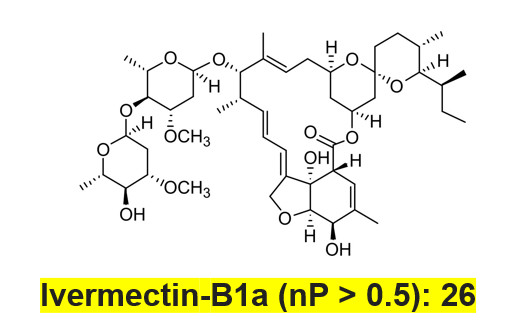
\includegraphics[width=0.4\linewidth]{C:/Users/stdso/Documents/USTH/Med/BioAct-Het-main/Output/Most/Ivermectin-B1a.jpg} \\
\end{center}

Notably, Ritonavir, Umifenovir, and Ivermectin-B1a are currently used to treat COVID-19, so patients taking these medications should be counseled on potential side effects and closely monitored.

% Discussion 
\section{Discussion}
In this section, the effectiveness of the proposed model is evaluated according to evaluation metrics. Resulting in 7 predicted side-effects drugs compared with the actual side-effect drugs in SIDER, the model is trustworthy or effective due to the average percentage of accuracy, prediction, F1-score, and recall is entirely greater than 85\% even though the quality paper was also proposed as a significantly accurate model due to almost all trained models that were greater than 75\%, except in MUV dataset. The usefulness in the real world is significantly applicable, particularly in discovering the future bioactivities of developed chemical compounds. COVID-19 is a mostly common disease, which can be used initially in this discovery to find potential drugs with at least side effects for future drug-taken dosage. The detail of toxicological and MUV datasets with a wide range of classes seem not to be enough to predict due to a large number of toxicology and similarity of chemical compounds, which hardly count with substances’ complexity. \\

COVID-19 is a common disease that caused numerous deaths, 7,040,264, in 2024 with a fifth rank compared with other pandemics. This makes scientists and researchers spend a long time investigating and conducting experiments, offering effective treatments and vaccines. With the different medications or newly introduced drugs, the prediction of bioactivities, such as side effects, is crucial before administering these marketed drugs to patients to ensure patient safety and combine future treatments to gain better outcomes in the decision-making process for use in clinical practice. Hydroxychloroquine is commonly known as a COVID-19 drug. However, severe side effects cause patients including cardiac toxicity. As a result, it stopped being released in most countries.\\

In the research, 24 potential COVID-19 drugs, such as Vancomycin or Paxlovid (Nirmatrelvir),  were collected after a long time investigation. These include antimalarial, antibiotic, or immunosuppressive drugs. It is an FDA-approved medication that has demonstrated efficacy in reducing hospitalization and serious consequences in COVID-19 patients. This method, which is in line with the compound-based strategy, will enable us to determine if the model can reliably forecast bioactivities and aid in the identification of novel drug bioactivities, particularly side effects, in the range of 0 to 1. \\

To obtain the representations of the chemical compounds, the pre-trained GCN-AttentiveFP model was used on SIDER. The BioAct-Het model is then given these representations, along with each side effect class representation that was derived. The Medical Dictionary for Regulatory Activities (MedDRA) provides a standardized medical language for classifying and coding medical history, clinical trial data, and adverse events in drug development and postmarket. This is where the side effects classes come from. Over 20,000 preferred words (PT), or low-level basic classes, are included in MedDRA and are arranged into 27 system organ groupings.\\

The results give 5 drugs with the least side effects including Paxlovid (Nirmatrelvir), Interferon-beta 1a, Linagliptin, Famotidine, and Hydroxychloroquine. However, Hydroxychloroquine, Linagliptin, and Famotidine are removed due to the report of a large number of side effects and unavailable COVID-19 drugs. Paxlovid (Nirmatrelvir) includes Injury, poisoning and procedural complications, Hepatobiliary Disorders, Metabolism and Nutrition Disorders, Investigations, Musculoskeletal and Connective Tissue Disorders, Gastrointestinal Disorders, Immune System Disorders, Reproductive System and Breast Disorders, General Disorders and Administration Site Conditions, Vascular Disorders, Blood and Lymphatic System Disorders, Skin and Subcutaneous Tissue Disorders, Infections and Infestations, Renal and urinary disorders, Nervous system disorders, Injury, poisoning, and procedural complications, Injury, poisoning and procedural complications; Interferon-beta 1a contains Metabolism and Nutrition Disorders, Investigations, Musculoskeletal and Connective Tissue Disorders, Gastrointestinal Disorders, Immune System Disorders, General Disorders and Administration Site Conditions, Vascular Disorders, Blood and Lymphatic System Disorders, Skin and Subcutaneous Tissue Disorders, Infections and Infestations, Respiratory, thoracic and mediastinal disorders, Psychiatric disorders, Renal and urinary disorders, Cardiac disorders, Nervous system disorders, Injury, poisoning and procedural complications.  Nevertheless, more investigation is required to completely comprehend potential side effects and assess the medication's safety and effectiveness in treating COVID-19 and other illnesses, as there have been few studies conducted on it.\\

The results give 5 drugs requiring careful use Ritonavir, Umifenovir, Cyclosporine, Prednisolone and Ivermectin-B1a. Three of these, such as Ritonavir, Umifenovir and Ivermectin-B1a, are known as COVID-19 drugs; however, the dosage of these drugs should be noticed to patients through prescriptions while obligatorily taking medicine.  \\

Based on the results of 25 drugs, some particular side effects consist of Immune System Disorders, Vascular Disorders, Nervous system disorders, Metabolism and Nutrition Disorders, Gastrointestinal Disorders and Musculoskeletal and Connective Tissue Disorders. Compared with 5 drugs least side effects, some particular side effects are included in table 3.\\

\begin{table}[h!]
  \centering
  \caption{Large 13x5 Table}
  \label{tab:large_table}
  \begin{tabular}{
    |c|>{\raggedright\arraybackslash}p{2.2cm}|
    >{\centering\arraybackslash}p{1.5cm}|
    >{\centering\arraybackslash}p{1.2cm}|
    >{\centering\arraybackslash}p{1.2cm}|}
    \hline
    \textbf{No.} & \textbf{Common Side Effects of the 25 Drugs}         & \textbf{Included in Top 5 with Least Side Effects} & \textbf{Paxlovid (Nirmatrelvir)} & \textbf{Interferon-beta 1a} \\ \hline
    1            & Immune System Disorders                              & Yes                                                & Yes                              & Yes                         \\ \hline
    2            & Vascular Disorders                                   & Yes                                                & Yes                              & Yes                         \\ \hline
    3            & Nervous System Disorders                             & Yes                                                & Yes                              & Yes                         \\ \hline
    4            & Metabolism and Nutrition Disorders                   & Yes                                                & Yes                              & Yes                         \\ \hline
    5            & Gastrointestinal Disorders                           & Yes                                                & Yes                              & Yes                         \\ \hline
    6            & Musculoskeletal and Connective Tissue Disorders      & Yes                                                & Yes                              & Yes                         \\ \hline
    7            & General Disorders and Administration Site Conditions & Yes                                                & Yes                              & Yes                         \\ \hline
    8            & Injury, Poisoning and Procedural Complications       & Yes                                                & Yes                              & Yes                         \\ \hline
    9            & Renal and Urinary Disorders                          & Yes                                                & Yes                              & Yes                         \\ \hline
    10           & Skin and Subcutaneous Tissue Disorders               & Yes                                                & Yes                              & Yes                         \\ \hline
    11           & Infections and Infestations                          & Yes                                                & Yes                              & Yes                         \\ \hline
    12           & Investigations                                       & Yes                                                & Yes                              & Yes                         \\ \hline
  \end{tabular}
\end{table}

% Conclusion
\section{Conclusion}
This study applies the BioAct-Het model to address the BCP problem. The main contributions of this study can be attributed to two key factors. Firstly, a novel approach of using Bio-Prof (Bioactivity class) to represent bioactivity classes as input of 25 investigated potentially marketed drugs. Moreover, the use of a heterogeneous SNN named BioAct-Het is motivated by the complexity and diversity of the relationships between chemical substances and bioactivity classes, resulting in embedding vectors. The model contains two branches for embedding compounds and bioactivity classes in similar concepts captured in a unified latent space. A limitation of this study is the focus on small molecules, which seems to be difficult in larger and complex molecules. Therefore, this factor should be considered in future research endeavors. The use of BioAct-Het as a pre-trained model in three strategies: Association-based, Bioactivity-based, and Compound-based approaches. If research time is extended, this model can be compared with other techniques. After considering under 25 potential drug inputs, Paxlovid (Nirmatrelvir) and Interferon-beta 1a (IFN-$\beta$1a) are recommended for use in COVID-19 treatment; however, this study should further investigate to test in vitro, in vivo, combined with the results of in silico.

\subsection*{Associated Content}
\subsubsection*{Data Availability Statement}
The data and code underlying this article are available publicly at \url{https://github.com/Xernnn/Bioact-Pred-Het-SNN}. However, data sets were derived from sources in the public domain.\\

\subsubsection*{Author Contributions}
\begin{table}[h!]
  \centering
  \caption{Author Contributions}
  \label{tab:Author Contributions}
  \begin{tabular}{|>{\centering\arraybackslash}m{2cm}|>{\centering\arraybackslash}m{3cm}|>{\centering\arraybackslash}m{3cm}|}
    \hline
    \textbf{Name}    & \textbf{Task}                                                                    & \textbf{Responsibility}                                                       \\ \hline
    Doan Huu Thanh   & Studied and conducted COVID-19 diseases and marketed drugs with SMILES structure & Supervised by Pham Hai Nam                                                    \\ \hline
    Nguyen Son       & Developed and implemented the method                                             & Interpreted results, wrote manuscript on LaTeX platform, administered project \\ \hline
    Le Mau Minh Phuc & Experimented and conceptualized using the Siamese Neural Network (SNN)           & Edited manuscript                                                             \\ \hline
    Pham Hai Nam     & Supervised Doan Huu Thanh, confirmed medical information related to COVID-19     & Interpreted results, wrote manuscript, administered project                   \\ \hline
  \end{tabular}
\end{table}

\bibliography{refs}
\clearpage

\onecolumn
% Appendices
\section*{Appendices}
\subsection*{\centering APPENDIX 1: Our Dataset}
\begin{table}[h]
  \centering
  \renewcommand{\arraystretch}{1.2}
  \begin{tabular}{|>{\bfseries}l|l|p{10cm}|}
    \hline
    \textbf{Drug}                            & \textbf{Chemical Compound}             & \textbf{SMILES Structure}                                                                                                                                                                                                                                                                                                                                                                                                                                                                                                                                                       \\
    \hline
    Vancomycin                               & C$_{66}$H$_{75}$Cl$_2$NO$_{21}$        & Cl.CN[C@H](CC(C)C)C(=O)N[C@@H]1[C@H](O)C2=CC=C(OC3=C(O[C@@H]4O \newline [C@H](CO)[C@@H](O)[C@H](O)[C@H]4O[C@H]4C[C@](C)(N)[C@H](O)[C@H] \newline (C)O4)C4=CC(=C3)[C@@H](NC(=O)[C@H](CC(N)=O)NC1=O)C(=O)N[C@@H]1C3 \newline =CC(=C(O)C=C3)C3=C(O)C=C(O)C=C3[C@H](NC(=O)[C@@H](NC1=O)[C@H](O) \newline C1=CC(Cl)=C(O4)C=C1)C(O)=O)C(Cl)=C2                                                                                                                                                                                                                                        \\
    \hline
    Cyclosporine                             & C$_{56}$H$_{77}$N$_{11}$O$_{11}$       & CC[C@@H]1NC(=O)[C@H]([C@H](O)[C@H](C)C\textbackslash C=C\textbackslash C)N(C)C(=O)[C@H](C(C)C) \newline N(C)C(=O)[C@H](CC(C)C)N(C)C(=O)[C@H](CC(C)C)N(C)C(=O)[C@@H](C)N \newline C(=O)[C@H](C)NC(=O)[C@H](CC(C)C)N(C)C(=O)[C@@H](NC(=O)[C@H](CC(C) \newline C)N(C)C(=O)CN(C)C1=O)C(C)C                                                                                                                                                                                                                                                                                          \\
    \hline
    Fingolimod                               & C$_{19}$H$_{33}$NO$_2$                 & Cl.CCCCCCCCC1=CC=C(CCC(N)(CO)CO)C=C1                                                                                                                                                                                                                                                                                                                                                                                                                                                                                                                                            \\
    \hline
    Remdesivir                               & C$_{27}$H$_{35}$N$_5$O$_8$P            & CCC(CC)COC(=O)C(C)NP(=O)(OCC1C(C(C(O1)(C\#N)C2=CC=C3N2N=CN=C3N)O) \newline O)OC4=CC=CC=C4                                                                                                                                                                                                                                                                                                                                                                                                                                                                                       \\
    \hline
    Oseltamivir                              & C$_{16}$H$_{31}$N$_3$O$_8$             & CCC(CC)OC1C=C(CC(C1NC(=O)C)N)C(=O)OCC                                                                                                                                                                                                                                                                                                                                                                                                                                                                                                                                           \\
    \hline
    Ritonavir                                & C$_{37}$H$_{47}$N$_3$O$_7$S            & CC(C)C1=NC(=CS1)CN(C)C(=O)NC(C(C)C)C(=O)NC(CC2=CC=CC=C2)CC(C(CC \newline 3=CC=CC=C3)NC(=O)OCC4=CN=CS4)O                                                                                                                                                                                                                                                                                                                                                                                                                                                                         \\
    \hline
    Molnupiravir                             & C$_{16}$H$_{16}$F$_3$N$_3$O$_5$        & CC(C)C(=O)OCC1C(C(C(O1)N2C=CC(=NC2=O)NO)O)O                                                                                                                                                                                                                                                                                                                                                                                                                                                                                                                                     \\
    \hline
    Paxlovid (Nirmatrelvir)                  & C$_{36}$H$_{45}$N$_5$O$_7$S            & CC1(C2C1C(N(C2)C(=O)C(C(C)(C)C)NC(=O)C(F)(F)F)C(=O)NC(CC3CCNC3=O)C \newline \#N)C                                                                                                                                                                                                                                                                                                                                                                                                                                                                                               \\
    \hline
    Guanfacine                               & C$_{9}$H$_{9}$Cl$_2$N$_3$O             & C1=CC(=C(C(=C1)Cl)CC(=O)N=C(N)N)Cl                                                                                                                                                                                                                                                                                                                                                                                                                                                                                                                                              \\
    \hline
    Liraglutide                              & C$_{166}$H$_{250}$N$_{40}$O$_{45}$S    & CCCCCCCCCCCCCCCC(=O)NC(CCC(=O)NCCCCC(C(=O)NC(CCC(=O)O)C(=O)NC \newline (CC1=CC=CC=C1)C(=O) NC(C(C)CC)C(=O) NC(C)C(=O)NC(CC2=CNC3=CC=CC= \newline C32)C(=O)NC(CC(C)C)C(=O)NC(C(C)C)C(=O)NC(CCCNC(=N)N)C(=O)NCC(=O) \newline NC(CCCNC(=N)N)C(=O)NCC(=O)O)NC(=O)C(C)NC(=O)C(C)NC(=O)C(CCC(=O)N) \newline NC(=O)CNC(=O)C(CCC(=O)O)NC(=O)C(CC(C)C)NC(=O)C(CC4=CC=C(C=C4)O)NC \newline (=O)C(CO)NC(=O)C(CO)NC(=O)C(C(C)C)NC(=O)C(CC(=O)O)NC(=O)C(CO)NC(=O) \newline C(C(C)O)NC(=O)C(CC5=CC=CC=C5)NC(=O)C(C(C)O)NC(=O)CNC(=O)C(CCC(=O)\newline O)NC(=O)C(C)NC(=O)C(CC6=CN=CN6)N)C(=O)O \\
    \hline
    Linagliptin                              & C$_{25}$H$_{28}$N$_7$O$_2$             & CC\#CCN1C2=C(N=C1N3CCCC(C3)N)N(C(=O)N(C2=O)CC4=NC5=CC=CC=C5C(=N\newline 4)C)C                                                                                                                                                                                                                                                                                                                                                                                                                                                                                                   \\
    \hline
    Baricitinib-Phosphate                    & C$_{16}$H$_{17}$N$_6$O$_3$S            & CCS(=O)(=O)N1CC(C1)(CC\#N)N2C=C(C=N2)C3=C4C=CNC4=NC=N3.OP(=O)(O)O                                                                                                                                                                                                                                                                                                                                                                                                                                                                                                               \\
    \hline
    Dexamethasone \newline -Sodium-Phosphate & C$_{22}$H$_{99}$FO$_5$P                & CC1CC2C3CCC4=CC(=O)C=CC4(C3(C(CC2(C1(C(=O)COP(=O)([O-])O-])O)C)O) \newline FC.[Na+].[Na+]                                                                                                                                                                                                                                                                                                                                                                                                                                                                                       \\
    \hline
    Tocilizumab                              & C$_{66}$H$_{76}$N$_{10}$O$_{16}$S      & CCNC(=O)[C@@H]1CC[C@@H]2C@@HCC[C@@H]2C1                                                                                                                                                                                                                                                                                                                                                                                                                                                                                                                                         \\
    \hline
    Remdesivir (Veklury)                     & C$_{27}$H$_{35}$N$_5$O$_8$P            & CCC(CC)COC(=O)C(C)NP(=O)(OCC1C(C(C(O1)(C\#N)C2=CC=C3N2N=CN=C3N)O) \newline O)OC4=CC=CC=C4                                                                                                                                                                                                                                                                                                                                                                                                                                                                                       \\
    \hline
    Anakinra                                 & C$_{76}$H$_{105}$N$_{19}$O$_{19}$S$_2$ & CC(C)C@HC(=O)NCC(=O)N                                                                                                                                                                                                                                                                                                                                                                                                                                                                                                                                                           \\
    \hline
    Chloroquine                              & C$_{18}$H$_{26}$ClN$_3$                & CCN(CC)CCCC(C)NC1=C2C=CC(=CC2=NC=C1)Cl                                                                                                                                                                                                                                                                                                                                                                                                                                                                                                                                          \\
    \hline
    Hydroxychloroquine                       & C$_{18}$H$_{26}$ClN$_3$O$_3$           & CCN(CCCC(C)NC1=C2C=CC(=CC2=NC=C1)Cl)CCO                                                                                                                                                                                                                                                                                                                                                                                                                                                                                                                                         \\
    \hline
    Famotidine                               & C$_{8}$H$_{15}$N$_3$O$_2$S             & C1=C(N=C(S1)N=C(N)N)CSCCC(=NS(=O)(=O)N)N                                                                                                                                                                                                                                                                                                                                                                                                                                                                                                                                        \\
    \hline
    Umifenovir                               & C$_{22}$H$_{28}$ClN$_3$O$_5$S          & CCOC(=O)C1=C(N(C2=CC(=C(C(=C21)CN(C)C)O)Br)C)CSC3=CC=CC=C3                                                                                                                                                                                                                                                                                                                                                                                                                                                                                                                      \\
    \hline
    Ivermectin-B1a                           & C$_{50}$H$_{76}$O$_{14}$               & CCC(C)C1C(CCC2(O1)CC3CC(O2)CC=C(C(C(C=CC=C4COC5C4(C(C=C(C5O)C)C \newline (=O)O3)O)C)OC6CC(C(C(O6)C)OC7CC(C(C(O7)C)O)OC)OC)C)C                                                                                                                                                                                                                                                                                                                                                                                                                                                   \\
    \hline
    Prednisolone                             & C$_{21}$H$_{26}$O$_5$                  & CC12CC(C3C(C1CCC2(C(=O)CO)O)CCC4=CC(=O)C=CC34C)O                                                                                                                                                                                                                                                                                                                                                                                                                                                                                                                                \\
    \hline
    Fluvoxamine                              & C$_{15}$H$_{21}$F$_3$N$_2$O$_2$        & COCCCCC(=NOCCN)C1=CC=C(C=C1)C(F)(F)F                                                                                                                                                                                                                                                                                                                                                                                                                                                                                                                                            \\
    \hline
    Baxdrostat                               & C$_{22}$H$_{25}$N$_3$O$_2$             & CCC(=O)NC1CCCC2=C1C=NC=C2C3=CC4=C(C=C3)N(C(=O)CC4)C                                                                                                                                                                                                                                                                                                                                                                                                                                                                                                                             \\
    \hline
  \end{tabular}
\end{table}
\newpage

\subsection*{\centering APPENDIX 2: The Bubble Charts and the Confusion Matrices of the 7 Selected Drugs}

\noindent
\begin{center}
  \begin{tabular}{p{0.35\textwidth} p{0.65\textwidth}}
    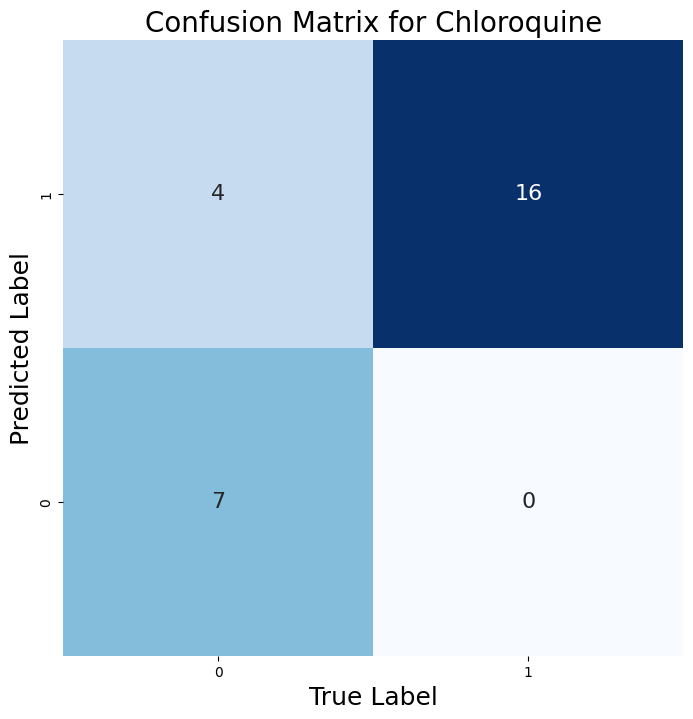
\includegraphics[width=\linewidth]{C:/Users/stdso/Documents/USTH/Med/BioAct-Het-main/Output/CF/Chloroquine_confusion_matrix.png} & 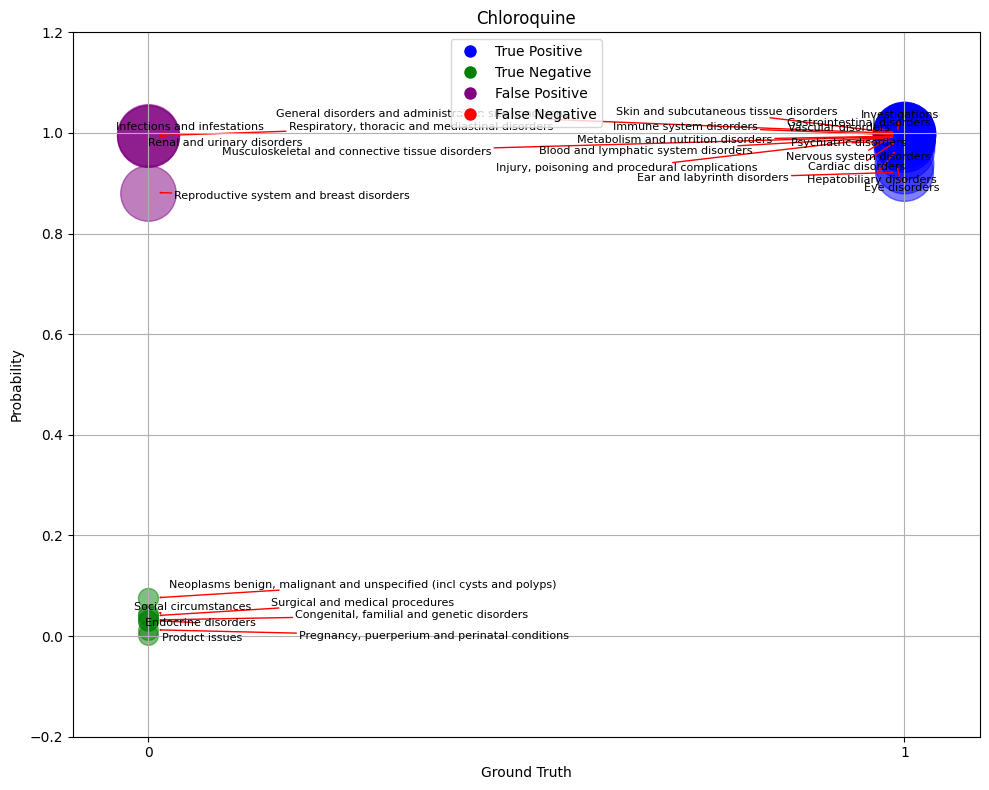
\includegraphics[width=\linewidth]{C:/Users/stdso/Documents/USTH/Med/BioAct-Het-main/Output/Bubble/Chloroquine_bubble_chart.png} \\
  \end{tabular}
  \vspace{10pt}
\end{center}

\noindent
\begin{center}
  \begin{tabular}{p{0.35\textwidth} p{0.65\textwidth}}
    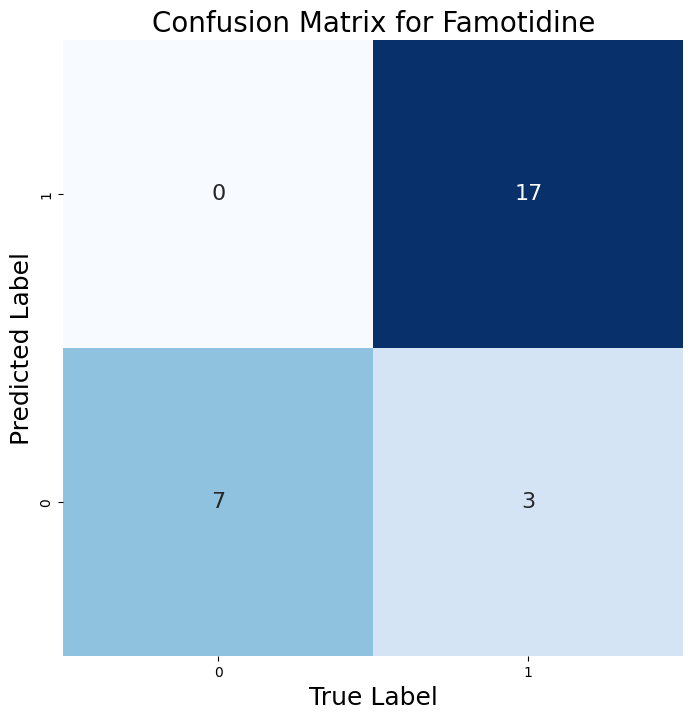
\includegraphics[width=\linewidth]{C:/Users/stdso/Documents/USTH/Med/BioAct-Het-main/Output/CF/Famotidine_confusion_matrix.png} & 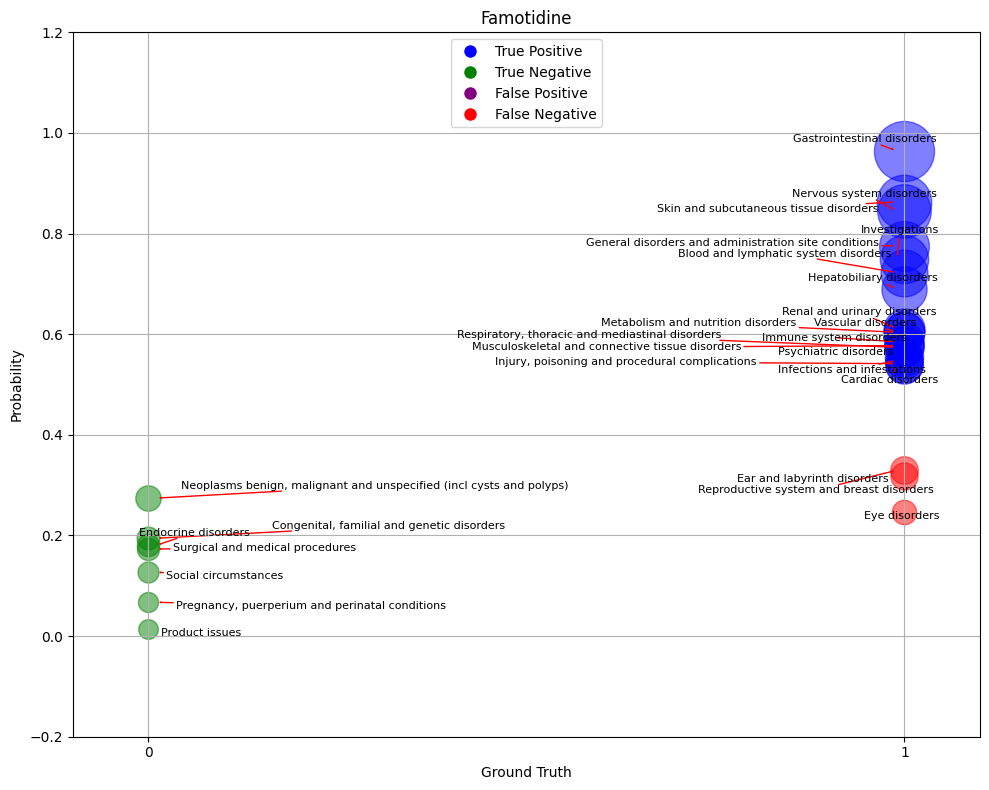
\includegraphics[width=\linewidth]{C:/Users/stdso/Documents/USTH/Med/BioAct-Het-main/Output/Bubble/Famotidine_bubble_chart.png} \\
  \end{tabular}
  \vspace{10pt}
\end{center}

\noindent
\begin{center}
  \begin{tabular}{p{0.35\textwidth} p{0.65\textwidth}}
    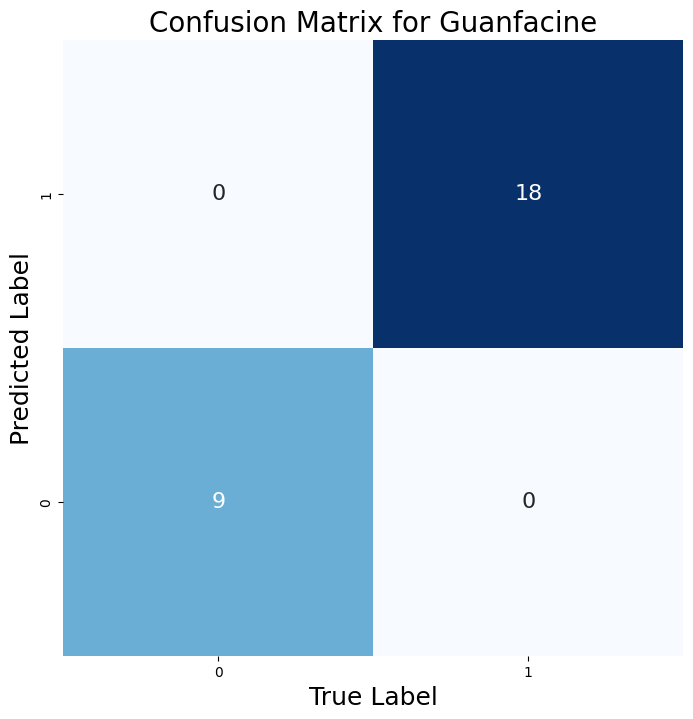
\includegraphics[width=\linewidth]{C:/Users/stdso/Documents/USTH/Med/BioAct-Het-main/Output/CF/Guanfacine_confusion_matrix.png} & 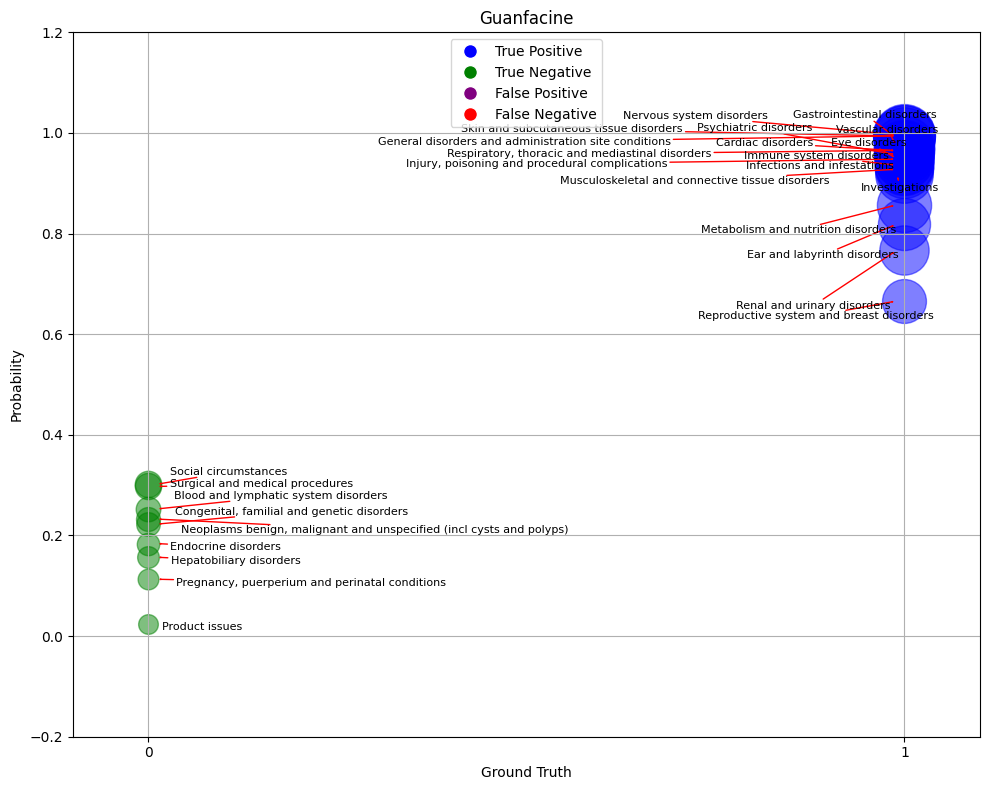
\includegraphics[width=\linewidth]{C:/Users/stdso/Documents/USTH/Med/BioAct-Het-main/Output/Bubble/Guanfacine_bubble_chart.png} \\
  \end{tabular}
  \vspace{10pt}
\end{center}

\noindent
\begin{center}
  \begin{tabular}{p{0.35\textwidth} p{0.65\textwidth}}
    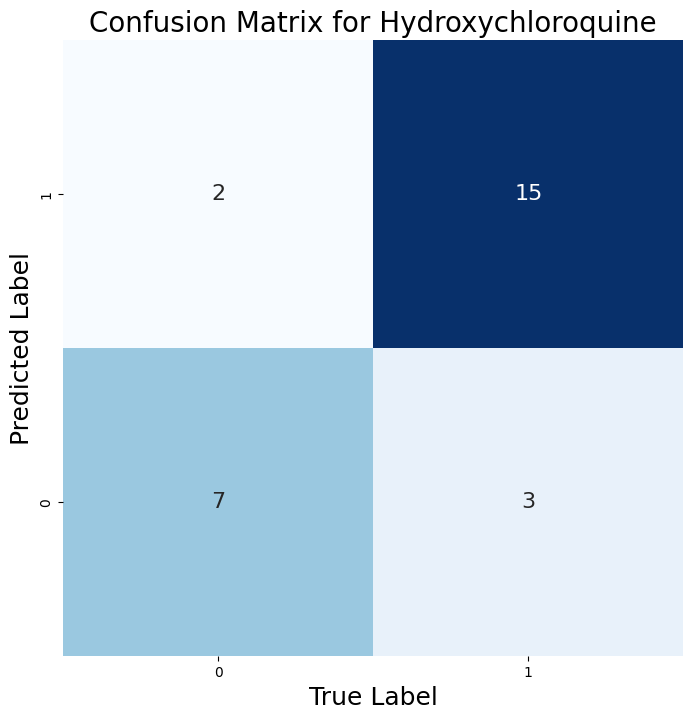
\includegraphics[width=\linewidth]{C:/Users/stdso/Documents/USTH/Med/BioAct-Het-main/Output/CF/Hydroxychloroquine_confusion_matrix.png} & 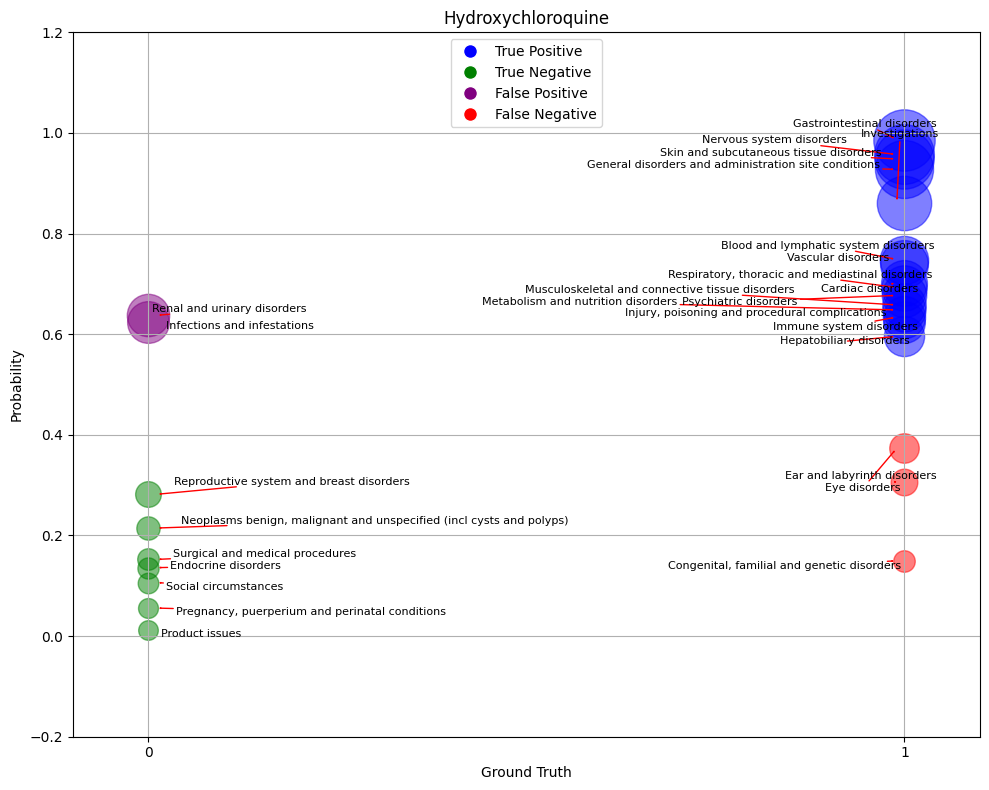
\includegraphics[width=\linewidth]{C:/Users/stdso/Documents/USTH/Med/BioAct-Het-main/Output/Bubble/Hydroxychloroquine_bubble_chart.png} \\
  \end{tabular}
  \vspace{10pt}
\end{center}

\noindent
\begin{center}
  \begin{tabular}{p{0.35\textwidth} p{0.65\textwidth}}
    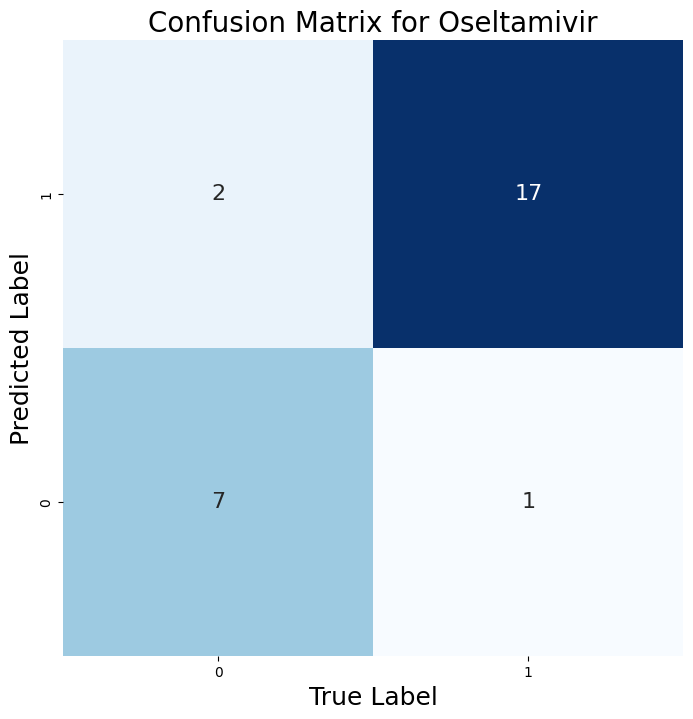
\includegraphics[width=\linewidth]{C:/Users/stdso/Documents/USTH/Med/BioAct-Het-main/Output/CF/Oseltamivir_confusion_matrix.png} & 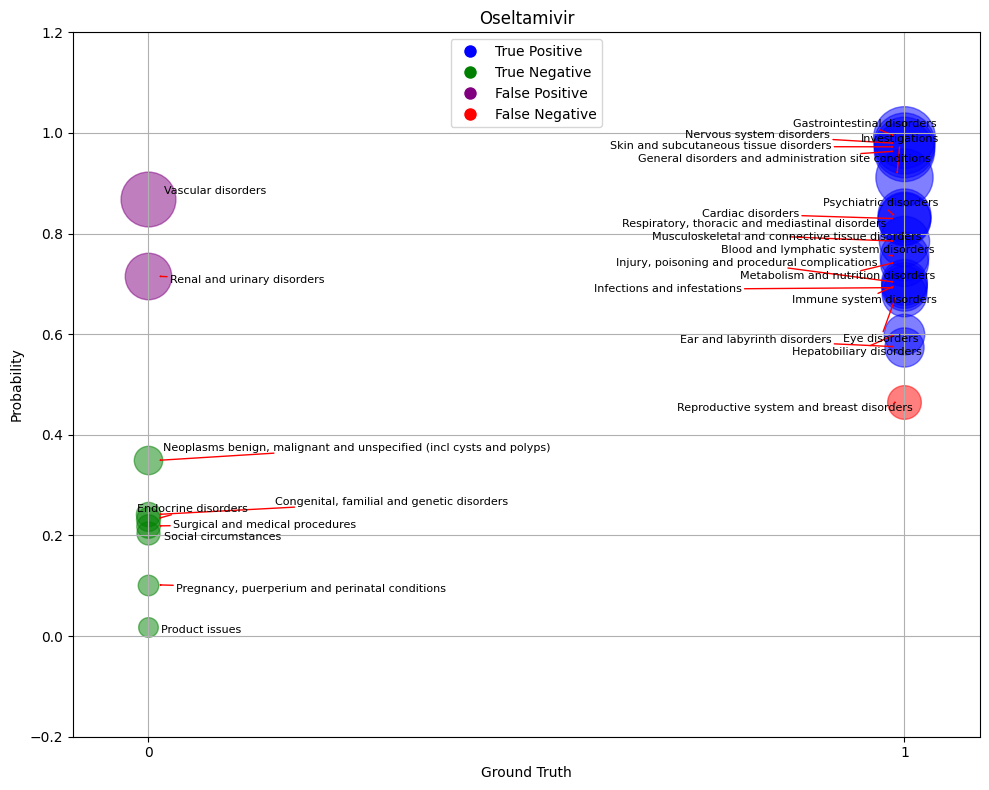
\includegraphics[width=\linewidth]{C:/Users/stdso/Documents/USTH/Med/BioAct-Het-main/Output/Bubble/Oseltamivir_bubble_chart.png} \\
  \end{tabular}
  \vspace{10pt}
\end{center}

\noindent
\begin{center}
  \begin{tabular}{p{0.35\textwidth} p{0.65\textwidth}}
    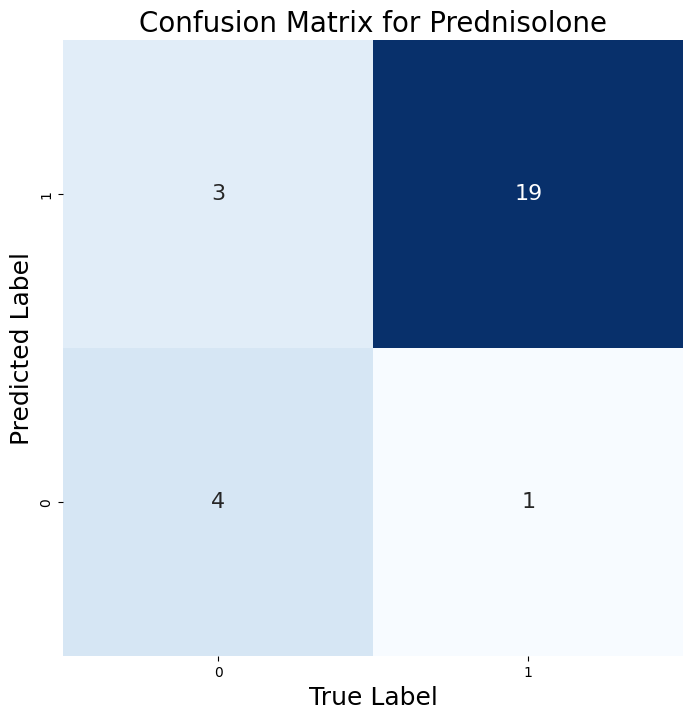
\includegraphics[width=\linewidth]{C:/Users/stdso/Documents/USTH/Med/BioAct-Het-main/Output/CF/Prednisolone_confusion_matrix.png} & 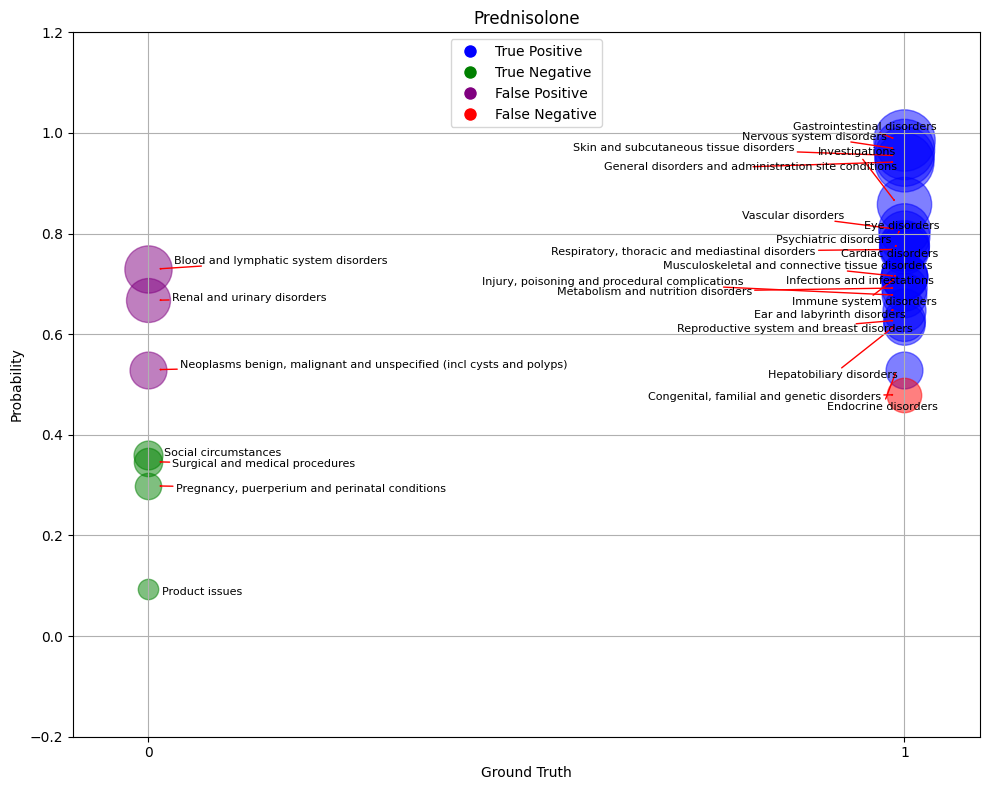
\includegraphics[width=\linewidth]{C:/Users/stdso/Documents/USTH/Med/BioAct-Het-main/Output/Bubble/Prednisolone_bubble_chart.png} \\
  \end{tabular}
  \vspace{10pt}
\end{center}

\end{document}